\section{Results: Systems Efficiency and Economics (RQ5)}
\label{sec:results_efficiency}

\subsection{LLM-Dependency Reduction Across the Resolution Ladder (E18)}
Layer E18 measured the five-tier ladder's traffic mix on 5{,}000 modeled queries per arm. Detection-gated routing raised the zero-LLM share from 10.48\% to 61.52\% (95\% CI [60.16, 62.86]). We report this decomposition explicitly rather than a single ``zero-LLM'' number: \textbf{deterministic advisory coverage} (\texttt{T1}+\texttt{T2}) is \DetAdvisoryCoverage{}, \textbf{safety/refusal handling} (\texttt{T0}+\texttt{T4}) is \SafetyRefusalHandling{}, and \textbf{LLM-dependent traffic} (\texttt{T3}) is \LLMDependent{}. Weighted mean latency falls from 1{,}247.93 ms to 546.15 ms (2.28$\times$), and serving cost from \$0.1785 to \$0.0767 per 1{,}000 queries. The distinction matters: the 10.48\% terminal-handling share is not ``answered without LLM''; it is refused or redirected.

\subsection{Stage-Level Latency Decomposition (E9)}
The E9 stage decomposition (analytical, modeled) localizes the latency story: deterministic routing 0.35 ms p95, deterministic lookup 0.42 ms, hybrid retrieval 28.5 ms, verification 3.8 ms, render 0.15 ms, and \emph{generation} 1{,}780 ms p95. Generation dominates latency by two orders of magnitude; verification does not. Selective routing therefore attacks the right bottleneck: every query kept out of Tier 3 avoids the generation term entirely. The deterministic tiers resolve in $\le$0.94 ms p95 (T0 0.42, T1 0.48, T2 0.58, T4 0.45). We label these figures as model-based decomposition values, not measured percentiles.

\subsection{Serving Cost and Cost per Correct Certified Safe Advisory (E20)}
Layer E20 builds a scenario-based cost model on the E18 traffic mix with Bangladesh A2P SMS rates (0.25 BDT) and local hosting. Per-query economics: app-online tiered \$0.000257, SMS fallback \$0.00234, commercial cloud LLM baseline \$0.00248 (i.e., \$0.2567 / \$2.34 / \$2.48 per 1{,}000). The app-online path is 89.65\% cheaper than the commercial baseline. We report these as scenario-based systems economics with the stated assumptions (6 queries/farmer/year, 50/30/20 app/offline/SMS mix, 120 BDT/USD), not as a national deployment forecast; the 16-million-farmer projection is deliberately excluded from the headline claims.

\subsection{Safety--Coverage--Latency Trade-off}
The Pareto narrative across the paper is: BAA trades coverage (97\% CAC at 33\% abstention; 84.56\% coverage at 1.26\% risk) for safety (0.0\% CUAR observed across E02, E05--E07, E28--E31, and E34) and wins latency on the deterministic share of traffic (2.28$\times$ weighted speedup; 3.8 ms vs 1.6--6.0 s baselines on the certified path). The trade-off is explicit and tunable through $\theta^*$; Section~\ref{sec:results_selective_reliability} shows the resulting risk--coverage frontier.

\begin{figure*}[!t]
\centering
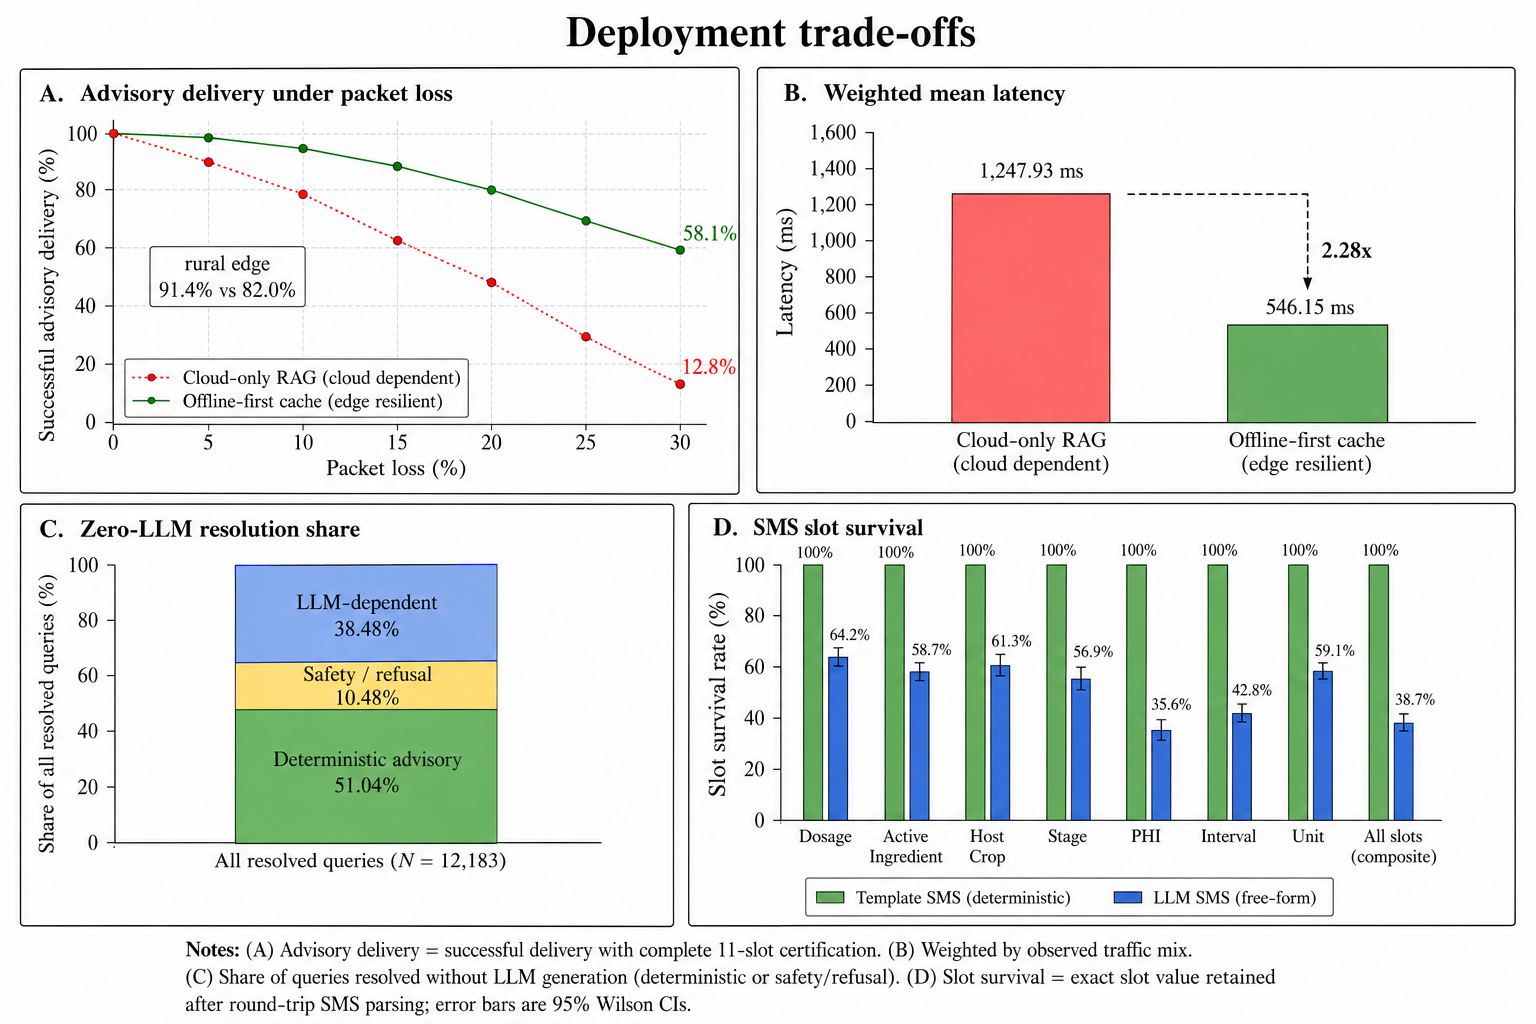
\includegraphics[width=0.92\textwidth,height=7.2cm,keepaspectratio]{figures/fig_6.png}
\caption{Deployment Trade-offs: Systems Efficiency, Connectivity Resilience, and Channel Economics. (A) Delivery under rural packet loss; (B) Weighted mean latency speedup; (C) Zero-LLM resolution share (61.5\% zero-cost); (D) 160-character Bengali SMS slot survival rate.}
\label{fig:deployment_tradeoffs}
\end{figure*}